% ------ headers globales y begin ---------------
\documentclass[11pt, a4paper, twoside]{article}
\usepackage{header_tp1}
\begin{document}{}
% -----------------------------------------------

\subsubsection{Descripción}\label{subsubsec:problema3-descripcion}

Este problema consiste en ubicar en un tablero la mayor cantidad de piezas
posibles siguiendo ciertas reglas.

\centerbf{Consideraciones}

\begin{itemize}   
	\item El tablero contiene $n \times m$ casilleros cuadrados, $n$ filas y $m$
	columnas.

	\item Piezas existentes: $1,...,n \times m$. (Cantidad total de
	piezas: $n \times m$).

	\item Una pieza es cuadrada y puede tener de $1$ a $4$ colores distintos.
	A cada lado $(sup, izq, der, inf)$ le corresponde un color.

	\item Las piezas no se pueden rotar.

	\item Colores posibles: $1,...,c$ ($c$ entero positivo).

	\item 2 piezas pueden ubicarse en casilleros adyacentes sólo si sus lados
	adyacentes tienen el mismo color. Podría ocurrir que no sea posible
	llenar completamente el tablero con las piezas existentes.

	%\item El contenido final de una casilla podría ser $1,...,n \times m$,
	%si se pudo colocar alguna ficha, o $0$ si quedara vacía.

	%\item Cantidad mínima de piezas que se pueden colocar en el tablero:
	%$(n \times m)/ 2$. (Se intercalan las piezas en el tablero).

  \item \textbf{El problema se deberá resolver utilizando la técnica de
    \red{\emph{Backtracking}} eligiendo algunas podas para mejorar los tiempos de
    ejecución del programa.}

\end{itemize}

\centerbf{Ejemplos}

\begin{ejemplo}

  Para un tablero de $3\times 3$ y uno de $2\times 2$, suponiendo un caso  donde
  ninguna ficha puede colocarse adyacente a otra, una de las posibles  soluciones
  sería la siguiente:

  En el tablero de $3\times 3$ se podrían colocar las fichas $1,2,3,4$  y $5$, y
  en el de $2\times 2$, las fichas $1$ y $2$.

  \begin{center}
      \begin{minipage}{0.2\textwidth}
          \begin{tabular}{|c|c|c|}
              \hline
               $1$ & $0$ & $2$ \\
              \hline
               $0$ & $3$ & $0$  \\
              \hline
               $4$ & $0$ & $5$ \\
              \hline
          \end{tabular}
      \end{minipage}
      \begin{minipage}{0.2\textwidth}
          \begin{tabular}{|c|c|}
              \hline
               $1$ & $0$ \\
              \hline
               $0$ & $2$ \\
              \hline
          \end{tabular}
      \end{minipage}
  \end{center}

\end{ejemplo}

\begin{ejemplo}

	Se tiene un tablero de $2\times 2$, los colores $1,2,3$
    y las piezas \textbf{1},\textbf{2},\textbf{3},\textbf{4} $:$

  \begin{center}
    \begin{minipage}{0.2\textwidth}
        \begin{tabular}{ |l l l|}
            \hline
                 & $1$     &       \\
            $3$  & \textbf{1} &   $2$ \\
                 & $2$     &       \\
            \hline
        \end{tabular}
    \end{minipage}
    \begin{minipage}{0.2\textwidth}
        \begin{tabular}{ |l l l|}
            \hline
                 & $3$     &       \\
            $2$  & \textbf{2} & $2$ \\
                 & $1$     &       \\
            \hline
        \end{tabular}
    \end{minipage}
    \begin{minipage}{0.2\textwidth}
        \begin{tabular}{ |l l l|}
            \hline
                 & $3$      &       \\
            $1$  & \textbf{2}  & $3$ \\
                 & $2$      &       \\
            \hline
        \end{tabular}
    \end{minipage}
    \begin{minipage}{0.2\textwidth}
        \begin{tabular}{ |l l l|}
            \hline
                 & $1$      &       \\
            $1$  & \textbf{4}  & $2$   \\
                 & $2$      &       \\
            \hline
        \end{tabular}
    \end{minipage}
   \end{center}

  En este caso, la cantidad máxima de piezas que se pueden colocar en el tablero es $3$. Entonces las posibles soluciones serían:

  \begin{center}
    \begin{minipage}{0.45\textwidth}
        \centering
        \begin{tabular}{ | l | l |}
            \hline
            \textbf{1}  & \textbf{2} \\
            \hline
            $0$  & \textbf{4} \\
            \hline
        \end{tabular}  \\
    \end{minipage}
    \begin{minipage}{0.45\textwidth}
        \begin{tabular}{ | l | l |}
            \hline
            $0$     & \textbf{2} \\
            \hline
            \textbf{3}  & \textbf{1} \\
            \hline
        \end{tabular} \\
    \end{minipage}
  \end{center}
\end{ejemplo}

\begin{paragraph}\

\centerbf{Algoritmos de backtracking (ideas y análisis general)}

El objetivo del problema es diseñar un algoritmo utilizando la técnica de
\textbf{backtracking}. El algoritmo de \textbf{backtracking} se puede concebir
como una técnica recursiva de recorrido de grafos\footnote{Quizás la oración
no está expresada de la mejor forma; al decir ``se puede concebir como...'' se
quiere dar a entender que no se está dando la \emph{definición estricta} de
backtracking, sino más bien una \emph{interpretación} de la misma. Se dio por
sobreentendido el hecho de que en su sentido más básico es ``una técnica de
resolución de problemas''; así, representando al ``universo de soluciones''
como un grafo, \textbf{y en el contexto del párrafo}, creemos que la idea que
se intenta exponer es válida.}, estableciendo un paralelismo entre <<el
universo de soluciones>>, y los nodos de un \textbf{grafo arbol n-ario}\footnote{
O incluso un grafo conexo con ciclos, en el caso de un problema muy mal modelado.}, en
donde cada nodo representa una solución posible, y $n$ representa la cantidad
máxima de soluciones distintas que pueden desprenderse a partir de realizar un
cambio determinado en la solución anterior (\emph{vecindad}). Además puede,
según el caso, ser interpretado como un árbol en donde cada nodo representa
\textbf{una solución o sub-solución no necesariamente ``válida''} (o \red{``bien formada''}), y en
donde sólamente \textbf{las hojas del árbol} serían
\red{\emph{soluciones ``correctamente formadas''}} (aunque no necesariamente factibles).

Podemos separar también el tipo de problema en dos casos: los
\darkgreen{\textbf{problemas de decisión}}, para los que es necesario que la
solución cumpla \darkgreen{ciertas condiciones particulares} determinados por la
denominada \darkgreen{\textbf{función de selección}}, y los
\blue{\textbf{problemas de optimización}}, los cuales son derivados de los
anteriores, y en donde se desea obtener \blue{la \textbf{``mejor''}} de las
soluciones válidas\footnote{ Es decir, las que cumplan con el criterio de
selección. Tener en cuenta que esto último no implica necesariamente la
existencia de funciones inválidas, sino que puede darse el caso en que el
criterio de selección admita que todas las soluciones a un problema determinado
son válidas, y por consiguiente simplemente se esté buscando obtener la mejor de
ellas.} en base a una \blue{\textbf{función objetivo}}, entendiendo a esta
última como <<\emph{la función que establece cuándo una solución es mejor que
otra}>>.

\end{paragraph}

\begin{paragraph}\

\centerbf{Pequeño ejemplo sobre las ideas anteriores}

Un ejemplo concreto de los párrafos anteriores sería un problema en el que se
nos pidiese encontrar una lista de 10 números del 1 al 20, tal que la lista sea
estrictamente creciente. Tendríamos entonces un \darkgreen{problema de
decisión}, en el que la \darkgreen{función de selección} estaría determinada por
las condiciones \emph{``que la lista sea estrictamente creciente''}, \emph{``que el número
esté entre 1 y 20''}, y \emph{``que el largo de la lista sea 10''}, es decir, en donde
tomaríamos como soluciones factibles a todas aquellas en que <<\textbf{lista[i] $<$
lista[i+1] y además $1 \leq $ lista[i] $ \leq 20$, y además $|$lista$|=
20$}>>\footnote{Se cometen abusos varios de notación para no ahondar en detalles
innecesarios.}. Si se agregara, además, la condición ``quiero de todas las listas
posibles la que maximice la sumatoria de cada uno de sus componentes'', me
encontraría entonces con un \bluebf{problema de optimización}.

En este ejemplo, entonces, una \darkgreenbf{solución factible} sería cualquiera que
cumpla con los \darkgreen{criterios de selección}, mientras que una \redbf{solución
correctamente formada}, es decir, aquellas que podrían pertenecer a las hojas de
un posible arbol / ``universo de soluciones'' (tal y como se menciona en el párrafo
introductorio), sería simplemente ``una lista de 10 números''\footnote{Esto último es
debatible si se considera el tamaño como un criterio de selección; en todo caso habría
que formalizar aún más y no viene al caso.}.

De esta forma, para el ejemplo anterior, se podría establecer un algoritmo en
que cada nodo interno del árbol de soluciones representase la
\textbf{subestructura} de una o más soluciones, sin llegar a ser una solución,
más concretamente, se podría asumir que el nodo raíz del arbol es una lista
vacía, y que cada hijo es una lista que contiene a los elementos de su padre, y
cuyo tamaño es superior al anterior en 1, de forma tal que es simple ver que: \emph{cada nodo
comparte una subestructura con sus nodos-hermanos heredada desde su nodo-padre,
y sólamente las hojas del arbol son soluciones}.


\end{paragraph}

\begin{paragraph}\

\centerbf{Análisis general}

Siguiendo la línea de pensamiento anterior al ejemplo, teniendo en cuenta todas
las ideas ya expuestas, calcular el gráfo completo del universo de soluciones
(factibles y no factibles) para este problema tendría una complejidad de
\bigO{n^n}, \emph{o incluso infinita} si no se estableciese una asbtracción
idónea al momento de transformar el universo de soluciones en un grafo. Además,
incluso luego de establecer una abstracción en la que el grafo no considerase,
por ejemplo, soluciones imposibles, el tamaño del grafo sigue siendo muy grande\footnote{
De orden factorial, como se expone luego.}. Por esta razón, para realizar esta tarea, se utiliza el
concepto de \emph{grafo implícito}, mediante el cual se establece matemáticamente la
composición del mismo, sin la necesidad de expresar cada una de sus componentes,
\textbf{sino a través de una descripción formal de sus nodos y aristas}, en
donde \textbf{cada nodo es una solución}, y \textbf{cada arista es la
transformación de una solución a una solución distinta dentro de su
\emph{vecindad}} de manera que, dado un caso de prueba particular, sea posible
recrearlo en el momento mismo en que se realiza el recorrido del grafo.

Para asegurar la correctitud según los criterios expuestos en el párrafo
anterior, es importante establecer una \emph{vecindad} tal que el universo de
soluciones tenga una subestructura adecuada para la realización de ``podas'', es
decir, que dados dos $nodos-hijos$ derivados de un mismo $nodo-padre$, se puedan
encontrar en estos características en común derivadas directamente de su padre;
más concretamente, el nodo padre debe representar una solución o subsolución
para la cual las funciones de selección y objetivo valúen de una forma idónea
con relación a sus hijos. Por ejemplo, si en un ejercicio de optimización se
lograse establecer un grafo de soluciones de tal forma que dado un nodo padre
sus nodos derivados tengan una valuación menor o igual en la función objetivo, y
se buscase la solución que la maximizara, sería fácil implementar entonces una
poda que, en el momento en que una subsolución alcance un valor menor al
deseado, \emph{corte} la rama de soluciones determinada por el susodicho nodo.

Para este algoritmo en particular, el problema planteado es de
\textbf{optimización}, ya que se desea obtener una solución válida (debe cumplir
ciertos requisitos, como que cada pieza coincida en sus colores con sus
aledañas), pero que además maximice la \blue{\textbf{función objetivo}},
definiendo a esta última como, dado un tablero determinado, la sumatoria de los
casilleros que contienen ficha.

% \begin{center}
% \textbf{Formalizando}
% \end{center}

% % - -
% % Definición de pieza

% \begin{notacion}
% Sea $\pi$ el conjunto formado por todas las 4-uplas de la forma
% \[
% p \in \pi \Leftrightarrow \{(\forall~{a, b, c, d} \in \nat)~\exists p = [a, b, c, d]\}
% \]
% \begin{flushright}
% decimos que $p \in \pi$ es una pieza.
% \end{flushright}
% \end{notacion}


% % - -
% % Definición del conjunto de piezas

% \begin{definicion}

% Dado el orden de piezas relativo a la entrada del problema, definimos el
% conjunto ordenado
% \[
% P = \{p_1, ..., p_n\}
% \]
% \begin{center}
% como el conjunto de todas las piezas posibles, de forma tal que 
% \end{center}
% \[
% \{i\geq 1\} \land \{(\forall{i<n})\ p_i < p_{i+1} \Leftrightarrow ``\textbf{pieza~i}"~es~anterior~a~``\textbf{pieza~i+1}"\}
% \]

% \end{definicion}
% \begin{notacion}

% $P[i]$ = $P_i$

% \end{notacion}


% % - -
% % Definición del tablero

% \begin{definicion}

% Sea $T \in \theta$ la sucesión finita de la forma 
% \[
% T = \{p_1, ..., p_n : \{i_{\geq 1}\in\nat\} \land \{(p_i \in \pi) \lor (p_i = ``\texttt{vacio}")\}\},
% \]

% $T$ representa a un tablero, y definimos a cada $T_i = p_i$ como <<el valor de
% la pieza ubicada en la posición $i$ del tablero, o ``\texttt{vacío}'' en el caso de que
% no hubiese ninguna>>

% \end{definicion}

% \begin{notacion}
% $T[i]$ = $T_i$, $\theta$ = <<conjunto de todos los posibles tableros>>
% \end{notacion}
% \begin{definicion}
% sea $t.lleno: \nat_{\geq 1} \rightarrow \nat$, tal que
% \[
%   \left\lbrace
%   \begin{array}{l}
%      t.lleno(i) = verdadero \text{ si } T[i] \neq \texttt{vacio} \\
%      t.lleno(i) = falso \text{ de lo contario} \\
%   \end{array}
%   \right.
% \]
% \end{definicion}

\begin{definicion}\label{def:ej3-objetivo}
Sean T el conjunto de todos los posibles tableros, 
definimos la función auxiliar 
$t.lleno: \nat_{\geq 1} \rightarrow [0,1]$, tal que
\[
  \left\lbrace
  \begin{array}{l}
     t.lleno(i) = 1 ~~~~~~~~ \text{ si T[i] contiene una pieza} \\
     t.lleno(i) = 0 ~~~~~~~~ \text{ de lo contario} \\
  \end{array}
  \right.
\]
La \blue{\textbf{función objetivo}} es, dado un tablero $t \in T$,
$f: T \rightarrow \nat$, de la forma
\blue{
\[
f(T) := \nsum_{i=1}^{\#casilleros}{ t.lleno \bigg( {\large T\left(i\right)} \bigg) }
\]
}
\end{definicion}

\end{paragraph}

\subsubsection{Planteamiento de resolución}\label{subsubsec:ej3-resolucion}

\begin{paragraph}\

\centerbf{Idea general}

La idea es aplicar el algoritmo de backtracking según las consideraciones
expuestas anteriormente. Para ello, recorreremos el tablero en un orden
determinado (de izquierda a derecha, de arriba a abajo), evaluando en cada
paso la ficha correspondiente a la posición donde se encuentra el recorrido:
de tal forma que en cada paso se evalúe la posición siguiente a la que se
evaluó en el paso anterior.

En cada paso del algoritmo se colocará una ficha, y luego se llamará
recursivamente a la función, probando así las fichas posteriores. Es
importante tener en cuenta que en cada llamada recursiva el algoritmo probará
con $M$ fichas, y se llamará recursivamente para cada una de ellas.

Es fácil ver que, \emph{en su versión más básica}, este comportamiento lleva a
tener una complejidad del orden de \bigO{M^N}, siendo $N=n*m$ la cantidad de
posiciones del tablero, y $M$ la cantidad de piezas, ya que se realizan $N$
iteraciones (una por cada posición del tablero), y en cada iteración se
prueban $M$ piezas, lo cual resulta en $\overbrace{M*M*M*...*M}^{N~veces} =
M^N$. Hay que tener en cuenta que esta forma de recorrer el universo de
soluciones está analizando también las soluciones no factibles, es decir las
que resultan imposibles, tal como ``colocar la misma pieza en todos los
casilleros''.

\end{paragraph}


\begin{paragraph}\

\centerbf{Poda: Función de Selección}\label{poda:ej3-seleccion}

La primer poda posible resulta totalmente trivial, ya que se trata de probar
en cada iteración sólamente las piezas que no se hayan colocado ya en el
tablero. Aunque esta poda es simple, y no es más que una aplicación incompleta
de las restricciones impuestas por la función de selección, se la menciona, ya
que de esta forma se reduce la complejidad a
\bigO{\overbrace{(M)*(M-1)*...*(M-(N-1))*(M-(N))}^{\text{N multiplicaciones,
restando una pieza en cada una}}}, es decir \bigO{\frac{M!}{(N-1)!}}
$\subseteq$ \bigO{M!}. Simplificando, diremos que esta cota reduce la
complejidad del orden exponencial \bigO{M^N} al orden factorial \bigO{M!}.

Sobre la misma poda anterior, se puede implementar una mejora, que es probar
en cada iteración sólamente las piezas cuyos colores sean coherentes con los
colores de las piezas que ya se encuentren colocadas en el tablero. Así, si
una posición tiene una pieza a la izquierda cuyo color derecho es verde, yo
debería poder colocar en esa posición sólamente las piezas cuyo color
izquierdo es verde. Esta última poda, tal y como está planteada, en realidad
se trata básicamente de \textbf{\red{reducir el recorrido del universo de
soluciones a ``las soluciones factibles''}}, es decir, las que generan un
tablero final válido. Conceptualmente no es distinta a la poda mencionada en
el párrafo anterior, sino que es más bien una extensión de la misma, ya que
las dos se encargan de \red{analizar en cada iteración la correctitud del
tablero en términos de la \textbf{función de selección}}. De hecho, esta poda
se encarga de \textbf{seleccionar sólamente las fichas que cumplan
\emph{estrictamente} con la función de selección}, mientras que la anterior
sólo aplica la restricción de forma parcial.

Es imposible, sin embargo, establecer \emph{a priori} una caracterización
precisa del orden de complejidad del algoritmo bajo las condiciones de esta
nueva poda, ya que la misma depende no solo del tamaño de entrada, sino del
contenido de la entrada. Puede darse, por ejemplo, el caso de una entrada en la
que todas las piezas tengan el mismo color en todos sus lados, lo cual
significaría que habría que probar todas las piezas en todas las posiciones, lo
cual conllevaría una complejidad de \bigO{M!}. También puede darse el caso en
que la disposición de la entrada sea de forma tal que luego de colocar la primer
pieza, sólo exista en cada paso una pieza posible, con lo cual la complejidad
sería del orden de \bigO{M * 1^{N-1}}, es decir \bigO{M}, lineal sobre la
cantidad de piezas. Por la razón expuesta en este párrafo diremos que, a pesar
de que según la disposición de la entrada la misma puede ser mucho menor, la
complejidad en el peor caso está igualmente acotada por \bigO{M!}.

Por todo lo antes expuesto, además, podemos asegurar que al final del
recorrido (es decir, luego de evaluar todas las hojas del árbol) se habrán
evaluado \emph{estrictamente} todas las \textbf{\red{soluciones factibles}},
ya que el algoritmo habrá recorrido en cada paso cada posición del tablero,
\textbf{\red{evaluando las piezas que cumplan estrictamente con el criterio de
selección}}.

\end{paragraph}

\begin{paragraph}\

\centerbf{Poda: Función Objetivo}

Como se expuso en párrafos anteriores, la solución brindada por el algoritmo
debe no solo cumplir con las condiciones de una determinada \red{función de
selección}, sino también maximizar cierta \blue{función objetivo (\emph{ref:
\ref{def:ej3-objetivo}})}, la cual depende de la cantidad de piezas dispuestas
en el tablero o, inversamente, de la cantidad de ``agujeros'', es decir,
posiciones en que no exista ninguna pieza.

Dado que las soluciones comparten una subestructura, en donde tomando un
determinado nodo $d$\footnote{Notación: llamémoslo <<subsolución>>} del arbol
de soluciones podemos asegurar que <<para todas las hojas para las que exista
un camino simple hacia ese nodo que contenga a los hijos de ese
nodo>>\footnote{O coloquialmente: que exista una ``relación de parentezco''
con ese nodo} la solución representada por esas hojas contiene a todas las
piezas que ya se encuentran determinadas en el nodo $d$, es válido afirmar que
si una deteriminada subsolución contiene cierta cantidad de ``agujeros'',
entonces todas sus soluciones derivadas también van a contener esos mismos
``agujeros''. Así, podemos decir que \emph{\red{la cantidad de agujeros de una hoja
es siempre mayor o igual a la cantidad de agujeros de su padre}}.

\begin{aclaracion}

Antes de continuar, vale hacer una aclaración ligada a la implementación, y es
que a efectos de abstraer este concepto, y mejorar la claridad del algoritmo
se consideró al ``agujero'' o ``casillero libre'' como otra pieza,
representada por la constante \texttt{PIEZA\_VACÍA} (es decir,
independientemente del \emph{tipo} con el que se elija representar a la pieza,
nos referiremos a esta pieza como \texttt{PIEZA\_VACÍA}).

\end{aclaracion}

A la luz de las consideraciones anteriores surge esta poda: el objetivo es
\red{\textbf{cortar una \emph{rama}\footnote{Es decir, una subsolución junto
con todas sus soluciones derivadas}}} en el momento en que se encuentra una
subsolución que, por su cantidad de piezas vacías, \red{\textbf{no es candidata a maximizar
la función objetivo}} (y ya que no lo es la subsolución, por las consideraciones
ya expuestas, se puede asumir que tampoco lo serán las soluciones derivadas de
ella).

\begin{center}
\begin{minipage}[h]{0.8\textwidth}
\begin{aclaracion}

A efectos de simplificar la explicación, procedemos a mencionar primero una
versión alternativa de esta poda, la cual quizás resulte más intuitiva. Dada la
recursión una determinada posición $n$, la cual define una subsolución $T_n$, es
fácil ver que si $T_n$ contiene $p$ \texttt{piezas no-vacías}, siendo $N$ la
cantidad de posiciones, se cumple que:

\begin{itemize}
  \item Las soluciones derivadas de $T_n$ contienen al menos $p$ piezas.
  \item Las soluciones derivadas de $T_n$ contienen a lo sumo $p + (N - n)$ piezas.
\end{itemize}

De esta forma, si uno va guardando la cantidad máxima de piezas encontradas, uno
puede cortar una rama cuando sabe que cualquier solución derivada de la misma
contendrá una cantidad menor.

\end{aclaracion}
\vspace{1em}
\end{minipage}
\end{center}

\begin{definicion}

Dada una determinada subsolución $T_n$, en donde $n$ representa a la posición
sobre la cual se encuentra la recursión, decimos que la misma contiene una
<<\emph{cantidad máxima posible de piezas vacías}>>, y esta es la cantidad de
piezas vacías que el tablero tendría en el peor caso. En otras palabras, \textbf{la
\red{cantidad máxima de piezas vacías} de un tablero $T_n$ es la cantidad de piezas
vacías que ya contiene la subsolución $T_n$ sumada a todas las piezas que aún
le faltan por poner en las sucesivas $T_{n+\dots}$}. Se asume para ello que el
peor caso posible es un tablero en donde todas las piezas $\in \{n+1,...,N\}$,
siguientes a la posición actual resulten incompatibles y, por lo tanto,
vacías. La cantidad de piezas de ese intervalo es, entonces, $N-n$.

\[
cantidadMaximaAgujeros(T_n) = cantidadAgujeros(T_n) + (N-n)
\]

\end{definicion}

\end{paragraph}

\begin{paragraph}{Implementación de la poda\\}

En un principio, podemos asumir que toda combinación posible de fichas es
\textbf{candidata a ser mejor solución}.

En cada paso recursivo, podemos analizar cuánto es el valor de
\texttt{cantidadMaximaAgujeros($T_n$)} para el tablero $T_n$ actual de ese
paso, y contrastarlo contra la \red{\textbf{menor cantidad máxima de agujeros
encontrada hasta el momento}}, la cual desde el punto de vista implementativo
es una variable ajena a la recursión (por ejemplo, una variable global, o un
parámetro de la propia recursión). Siempre que se encuentre una <<cantidad
máxima de agujeros>> menor a la global, se actualizará el valor de la segunda.
Para ello, se inicializará esta última variable con el valor del peor caso
posible ($N \times M$), es decir el de un tablero en donde todas las piezas
sean vacías.

Como dijimos anteriormente, \textbf{dada una subsolución \redbf{$S$}}, podemos
asegurar que todas sus soluciones derivadas tendrán al menos la misma cantidad
de piezas vacías. Utilizando esta última consideración, dada una subsolución
con \redbf{$k_{S}$} piezas vacías, y sea \darkgreenbf{$X_{min}$} la
\texttt{menor cantidad máxima de agujeros encontrada hasta el momento}, de tal
forma que \darkgreenbf{$X_{min}$} $<=$ \redbf{$k_{S}$}, podemos afirmar que la
cantidad de \texttt{piezas no vacías} de cualquier solución derivada de esa
\redbf{subsolución $k_{S}$} no es en particular \textbf{mayor} a la cantidad
de \texttt{piezas no vacías} del resto de las soluciones, ya que por lo antes
expuesto sabemos que dada la existencia de \darkgreenbf{$X_{min}$} existe al
menos una subsolución \darkgreenbf{$T$} tal que su cantidad máxima de piezas
vacías es exactamente \darkgreenbf{$k_{T} = X_{min}$} $<=$ \redbf{$k_{S}$}, lo
cual es equivalente a afirmar que la \darkgreenbf{\emph{cantidad mínima de
piezas no vacías de cualquier solución derivada de T}} es \darkgreenbf{$N -
k_{T} = N - X_{min}$}, y dado que \darkgreenbf{$k_{T}$} $<=$ \redbf{$k_{S}$}
se deduce que \darkgreenbf{$(-K_{T})$} $>=$ \redbf{$(-k{S})$}, de lo que
finalmente se desprende que $T - K_{T} >= T - k_{S}$ es decir \blue{la
\emph{cantidad mínima de piezas no vacías de cualquier solución derivada} de
\darkgreenbf{$T$} es mayor o igual a la \emph{cantidad mínima de piezas no
vacías de cualquier solución derivada} de \redbf{$S$}}.

De todo lo anterior surge que mediante esta poda se logra descartar ciertas
soluciones, cuando se está seguro de que las mismas no maximizan la función
objetivo o, en caso de hacerlo, de que ya se encontró\footnote{o al menos,
implícitamente, se tiene certeza de su existencia} al menos una solución que
la maximice de igual o mejor forma.

\begin{corolario}

Dado un tablero de \textbf{$T$ posiciones}, y \textbf{$T$ piezas cualesquiera},
sin tomar a consideración sus colores, podemos asegurar que la \textbf{cantidad
mínima de piezas} que podemos colocar en el mismo es de $\lceil{T/2}\rceil$, de
forma tal que las piezas se distribuyan tal y como los casilleros de un mismo
color en un \texttt{Tablero de Ajedrez}. Esto es así debido a que esta
distribución nos asegura que en las posiciones indicadas ninguna pieza tiene
contacto inmediato con cualquier otra pieza, por lo que no existe riesgo de
incompatibilidad. De forma recíproca, podemos también asegurar que la
\textbf{menor cantidad máxima de agujeros} que el tablero puede llegar a
contener es de a lo sumo $\lfloor{T/2}\rfloor$. Estos valores pueden ser
utilizados, entonces, como inicialización de las variables globales mencionadas
en la explicación de la poda.

Esta misma observación nos permite, también, afirmar que dado un tablero
cualquiera existe al menos una solución factible.

\end{corolario}

\end{paragraph}

%La idea base es ir llenando el tablero en cierto orden, probando colocar en cada
%casillero piezas que no rompan las reglas, y analizando la cantidad total de
%piezas del tablero que hayan sido cubiertas. Se debe guardar de alguna forma la
%combinación de piezas que haya cubierto más casilleros.\\ Consideramos dejar un
%casillero libre como colocar la pieza representada por el 0. En este problema
%una solución candidata o rama es una sucesión de piezas (que puede o no incluir
%el 0), que van cubriendo el tablero.\\ Una primera decisión que se tomó fue
%guardar una estructura piezasPorColores que para cada par de colores (x, y)
%guarda una lista con todos las piezas que tienen como color superior e izquierdo
%x e y, respectivamente. Vamos recorriendo el tablero en cada fila de izquierda a
%derecha, desde la fila superior hasta la inferior. De este modo una pieza es
%legal en una posición si su color izquierdo es igual al color derecho de la
%pieza a su izquierda (de existir), y su color superior es igual al color
%inferior de la pieza ubicada arriba (de existir). Podemos obtener las piezas
%candidatas que cumplen con esa restricción de colores en piezasPorColores. De
%este modo nos aseguramos que todas las piezas por las que nos vamos ramificando
%mantienen las restricciones del tablero. Evitamos así tener que iterar sobre
%todas las piezas verificando si cumplen la restricción.\\
%Una poda muy sencilla pero muy útil que se 
%implementó fue dejar de buscar soluciones cuando encontramos una solución que
%cubre todo el tablero. \\
%A continuación se detalla otra poda. Vamos
%llevando cuenta de los huecos que dejamos en el tablero. Si hemos dejado tantos
%huecos como para que, aun llenando correctamente lo que queda del tablero, no
%alcanza para superar la mejor solución encontrada hasta el momento, abandonamos
%la rama.\\

%Al comenzar la búsqueda sabemos que por lo menos vamos a
%poder llenar la mitad de los casilleros del tablero. Ésto siempre se puede
%conseguir si visualizamos nuestro tablero como uno de ajedrez y ponemos las
%piezas en los casilleros negros. Ningún par de piezas compartiría lado. 

\newpage
\subsubsection{Detalle del algoritmo}
\begin{paragraph}\
\begin{verbatim}

Tablero backtrack( Tablero t, IndiceDePiezas ip, int posicion )
{
  Tablero mejorTablero = NULL;
  if ( t.yaEncontreUnTableroMejor( posicion ) )
  {
    return mejorTablero;
  }
  IteradorIndiceDePiezas it = ip.dameIterador( posicion );
  // Me fijo si estoy antes de la ultima posicion
  if ( posicion < t.cantidadDePosiciones - 1 )
  {
    while ( it.hayPiezasPosibles() )
    {
      // Si es asi, entonces llamo a backtrack para cada pieza posible
      t.ponerPiezaEnPosicion( *it, posicion );
      ip.marcarPiezaUtilizada( it );
      // Hago recursion en el backtracking
      Tablero otroTablero = NULL;
      otroTablero = backtrack( t, ip, posicion + 1 );
      if ( !mejorTablero )
      {
        mejorTablero = otroTablero;
      }
      else
      {
        if ( !otroTablero )
        {
          ip.marcarPiezaDisponible ( it );
          // Si la recursion me devolvio un puntero a nulo termino el BT
          break;
        }
        else
        {
          if ( mejorTablero < otroTablero )
          {
            mejorTablero = otroTablero;
          }

        }
      }
      ip.marcarPiezaDisponible ( it );
      it++;
    }
  }
  else
  {
    // (si estoy en la ultima posicion del tablero)
    // Intento colocar la ultima pieza
    if ( it.hayPiezasPosibles() )
    {
      t.ponerPiezaEnPosicion( *it, posicion );
    }
    // Creo una copia del tablero final
    mejorTablero = new Tablero( t );
    // Pongo una pieza transparente en el lugar donde puse (o no) una pieza
    t.ponerPiezaEnPosicion( PIEZA_VACIA, posicion );
  }
  return *mejorTablero;
}
\end{verbatim}

\end{paragraph}


\newpage

\subsubsection{Justificación formal de correctitud}
Se demostró la correctitud de este algoritmo y sus podas en la propia descripión
del mismo: por un lado afirmamos que la \textbf{correctitud de un algoritmo
genérico de Backtracking}, en su sentido más básico, \textbf{resulta trivial},
amparandonos en la propia definición de \textbf{Backtracking}, siendo que el
algoritmo ``\emph{analiza el universo de soluciones}''. Luego, durante la
descripción de las dos podas implementadas, se demostró que, en el caso de la
poda relacionada con la <<Función de Selección>> se estaban eliminando las
soluciones no factibles, las cuales iban a ser de todas formas descartadas por
el algoritmo durante el recorrido de las soluciones, y que en el caso de la poda
relacionada con la <<Función Objetivo>> se estaban eliminando todas aquellas
soluciones para las que dadas las condiciones de la subestructura implementada
se podía preveer que no iban a cumplir con el objetivo de maximizar la función
requerida.

\subsubsection{Cota de complejidad temporal}

La complejidad de este algoritmo pertenece a la familia de \bigO{M!}, en donde M
es la cantidad de piezas (contando la pieza vacía). Esto está demostrado en la
sección \subsubsecref{ej3}{resolucion}, en el apartado de la poda relacionada
con la función de selección.

\subsubsection{Verificación mediante casos de prueba}

A continuación presentamos distintas instancias que sirven para verificar que el
programa funciona correctamente.

\begin{center}
\begin{minipage}{0.5\textwidth}
	\begin{tabular}{llll}
		Input  \\
		\hline
		n       & m       & c       &         \\
		$sup_1$ & $izq_1$ & $der_1$ & $inf_1$ \\
		\vdots & \vdots   & \vdots  & \vdots  \\
		$sup_{nxm}$ & $izq_{nxm}$ & $der_{nxm}$ & $inf_{nxm}$ \\ 
	\end{tabular} \\  
\end{minipage}
\begin{minipage}{0.5\textwidth}	
	\begin{tabular}{lll}
		Output  \\
		\hline
		$x_1$ & \dots & $x_m$ \\
		\vdots&       & \vdots \\
		$x_n$ & \dots & $x_{nxm}$ \\
		 \\
	\end{tabular} \\
\end{minipage} \\

\begin{minipage}{0.5\textwidth}
\begin{itemize}
	\item{$n$}: \#filas.
	\item{$m$}: \#columnas.
	\item{$c$}: \#colores.
	\item{$sup_i$, $izq_i$, $der_i$, $inf_i$}: colores (entre 1 y c) de los lados de la pieza $i$.
	\item{$x_i$}: número de la pieza en la casilla $i$ del tablero. (``0'' si no hay ninguna pieza).
\end{itemize}
\end{minipage}
\end{center}



Separamos en casos y mostramos ejemplos para cada uno: 
\begin{itemize}
\item Todas las piezas son iguales:
	\begin{itemize}
		\item El tablero se completa. \\
			\begin{minipage}{0.2\textwidth}
				\begin{tabular}{l}
					Input  \\
					\hline
					$2$ $2$ $1$       \\
					$1$ $1$ $1$ $1$ \\
					$1$ $1$ $1$ $1$ \\
					$1$ $1$ $1$ $1$ \\
					$1$ $1$ $1$ $1$ \\
				\end{tabular} \\  
			\end{minipage}
			\begin{minipage}{0.2\textwidth}	
				\begin{tabular}{l}
					Output  \\
					\hline
					$1$ $2$ \\
					$3$ $4$ \\
					\\
					\\
					\\
				\end{tabular} \\
			\end{minipage} \\
			\begin{minipage}{0.2\textwidth}
				\begin{tabular}{l}
					Input  \\
					\hline
					$2$ $2$ $2$       \\
					$1$ $2$ $2$ $1$ \\
					$1$ $2$ $2$ $1$ \\
					$1$ $2$ $2$ $1$ \\
					$1$ $2$ $2$ $1$ \\
				\end{tabular} \\  
			\end{minipage}
			\begin{minipage}{0.2\textwidth}	
				\begin{tabular}{l}
					Output  \\
					\hline
					$1$ $2$ \\
					$3$ $4$ \\
					\\
					\\
					\\
				\end{tabular} \\
			\end{minipage} \\
			
			En estos ejemplos el tablero se completaría colocando las $4$ piezas de cualquier forma. No hay restricciones. \\

		\item El tablero tiene la mínima cantidad de piezas (($n \times m)/2$).\\
		
		    \begin{minipage}{0.2\textwidth}
				\begin{tabular}{l}
					Input  \\
					\hline
					$2$ $2$ $2$       \\
					$1$ $2$ $1$ $2$ \\
					$1$ $2$ $1$ $2$ \\
					$1$ $2$ $1$ $2$ \\
					$1$ $2$ $1$ $2$ \\
				\end{tabular} \\  
			\end{minipage}
			\begin{minipage}{0.2\textwidth}	
				\begin{tabular}{l}
					Output  \\
					\hline
					$1$ $0$ \\
					$0$ $2$ \\
					\\
					\\
					\\
				\end{tabular} \\
			\end{minipage} 
			\begin{minipage}{0.2\textwidth}	
				\begin{tabular}{l}
					Output  \\
					\hline
					$0$ $1$ \\
					$2$ $0$ \\
					\\
					\\
					\\
				\end{tabular} \\
			\end{minipage} \\
			
			En este caso sólo se pueden colocar las piezas intercaladas. Se podrían tomar $2$ piezas cualesquiera para la solución (Ej: piezas $3$ y $4$). \\
			
	\end{itemize}
\item Todas las piezas son diferentes:
     \begin{itemize}
		\item El tablero se completa. \\
		
		    \begin{minipage}{0.2\textwidth}
				\begin{tabular}{l}
					Input  \\
					\hline
					$3$ $3$ $8$     \\
				    $8$ $2$ $6$ $2$ \\ 
					$1$ $1$ $2$ $4$ \\
					$1$ $2$ $7$ $5$ \\
					$3$ $4$ $4$ $6$ \\
					$4$ $4$ $3$ $7$ \\
					$5$ $3$ $6$ $8$ \\
					$6$ $4$ $1$ $2$ \\
					$7$ $1$ $2$ $7$ \\
					$8$ $8$ $1$ $3$ \\
				\end{tabular} \\  
			\end{minipage}
			\begin{minipage}{0.2\textwidth}	
				\begin{tabular}{l}
					Output  \\
					\hline
					$9$ $2$ $3$ \\
					$4$ $5$ $6$ \\
					$7$ $8$ $1$ \\
					\\
					\\
					\\
					\\
					\\
					\\
					\\
				\end{tabular} \\
			\end{minipage} \\
		
		\item El tablero tiene la mínima cantidad de piezas (($n \times m)/2$). \\
		
			\begin{minipage}{0.2\textwidth}
				\begin{tabular}{l}
					Input  \\
					\hline
					$2$ $2$ $3$     \\
					$2$ $3$ $2$ $2$ \\
					$1$ $1$ $2$ $2$ \\
					$1$ $3$ $2$ $2$ \\
					$2$ $1$ $2$ $2$ \\
				\end{tabular} \\  
			\end{minipage}
			\begin{minipage}{0.2\textwidth}	
				\begin{tabular}{l}
					Output  \\
					\hline
					$1$ $0$ \\
					$0$ $2$ \\
					\\
					\\
					\\
				\end{tabular} \\
			\end{minipage} 
			\begin{minipage}{0.2\textwidth}	
				\begin{tabular}{l}
					Output  \\
					\hline
					$0$ $1$ \\
					$2$ $0$ \\
					\\
					\\
					\\
				\end{tabular} \\
			\end{minipage} \\
		
		En este caso sólo se pueden colocar las piezas intercaladas. Se podrían tomar $2$ piezas cualesquiera para la solución (Ej: piezas $3$ y $4$). \\
		
		\item El tablero no se completa pero se llena más que el mínimo posible. \\
		
			\begin{minipage}{0.2\textwidth}
				\begin{tabular}{l}
					Input  \\
					\hline
					$2$ $2$ $3$     \\
					$1$ $2$ $1$ $1$ \\
					$1$ $1$ $1$ $2$ \\
					$2$ $2$ $3$ $2$ \\
					$3$ $2$ $3$ $3$ \\
				\end{tabular} \\  
			\end{minipage}
			\begin{minipage}{0.2\textwidth}	
				\begin{tabular}{l}
					Output  \\
					\hline
					$1$ $2$ \\
					$0$ $3$ \\
					\\
					\\
					\\
				\end{tabular} \\
			\end{minipage} \\
	\end{itemize}
	
\item Existe alguna pieza diferente al resto: 
     \begin{itemize}
		\item El tablero se completa. \\
		
			\begin{minipage}{0.2\textwidth}
				\begin{tabular}{l}
					Input  \\
					\hline
					$2$ $2$ $2$     \\
					$2$ $2$ $1$ $2$ \\
					$2$ $2$ $1$ $2$ \\
					$2$ $1$ $2$ $2$ \\
					$2$ $1$ $2$ $2$ \\
				\end{tabular} \\  
			\end{minipage}
			\begin{minipage}{0.2\textwidth}	
				\begin{tabular}{l}
					Output  \\
					\hline
					$1$ $3$ \\
					$2$ $4$ \\
					\\
					\\
					\\
				\end{tabular} \\
			\end{minipage} \\
		
		\item El tablero tiene la mínima cantidad de piezas (($n \times m)/2$). \\
		
			\begin{minipage}{0.2\textwidth}
				\begin{tabular}{l}
					Input  \\
					\hline
					$2$ $2$ $3$     \\
					$2$ $2$ $1$ $2$ \\
					$3$ $3$ $3$ $1$ \\
					$3$ $2$ $1$ $1$ \\
					$2$ $2$ $1$ $2$ \\
				\end{tabular} \\  
			\end{minipage}
			\begin{minipage}{0.2\textwidth}	
				\begin{tabular}{l}
					Output  \\
					\hline
					$1$ $0$ \\
					$0$ $4$ \\
					\\
					\\
					\\
				\end{tabular} \\
			\end{minipage} 
			\begin{minipage}{0.2\textwidth}	
				\begin{tabular}{l}
					Output  \\
					\hline
					$0$ $1$ \\
					$2$ $0$ \\
					\\
					\\
					\\
				\end{tabular} \\
			\end{minipage} \\
		
		En este caso sólo se pueden colocar las piezas intercaladas. Se podrían tomar $2$ piezas cualesquiera para la solución (Ej: piezas $3$ y $4$). \\
		
		\item El tablero no se completa pero se llena más que el mínimo posible. \\
		
			\begin{minipage}{0.2\textwidth}
				\begin{tabular}{l}
					Input  \\
					\hline
					$2$ $2$ $3$     \\
					$2$ $2$ $1$ $2$ \\
					$3$ $2$ $3$ $1$ \\
					$3$ $1$ $3$ $2$ \\
					$2$ $2$ $1$ $2$ \\
				\end{tabular} \\  
			\end{minipage}
			\begin{minipage}{0.2\textwidth}	
				\begin{tabular}{l}
					Output  \\
					\hline
					$1$ $3$ \\
					$0$ $4$ \\
					\\
					\\
					\\
				\end{tabular} \\
			\end{minipage} \\
		
	\end{itemize}
		
\end{itemize}

Ejecutamos el programa con los distintos ejemplos y se llegó a la solución
esperada. Por lo tanto, podemos concluir que el comportamiento del programa es
correcto.

\clearpage

\subsubsection{Medición empírica de la performance}

Para realizar las pruebas de tiempo se nos presentaron varias complicaciones.
Dado que la complejidad del algoritmo implementado es exponencial, el tiempo de
ejecución se vuelve inmenso ante tamaños de entrada relativamente pequeños. Por
ejemplo, dado un tamaño de entrada de $n=4$, $m=4$, $c=10$, tenemos una cantidad
de fichas $M=(n*m)+1=17$, y dado que la complejidad del algoritmo es \bigO{M!},
esto es equivalente a afirmar que existe una constante $k$ para la cual a partir
de un $n_0$ nuestro algoritmo está acotado superiormente por $k*(M!)$. Puesto
que decimos que este $M!$ en realidad surge de la cantidad de soluciones
analizadas, si imaginásemos que el procesador demorase un ciclo de clock en
calcular una solución\footnote{Es el mínimo valor que le podemos asignar sin
involucrarnos demasiado con la arquitectura/microarquitectura del procesador},
averiguar todo el universo de soluciones bajo las condiciones expuestas en este
ejemplo tardaría a lo sumo $17!$ ciclos de clock o, suponiendo un procesador de
3GHz\footnote{Es decir, $3*2^30 ciclos por segundo.$}, unos 110419 segundos
(aproximadamente media hora).


Debido a lo expuesto anteriormente, nos resultó casi imposible medir el
comportamiento del algoritmo para tamaños de tablero muy grandes. Se realizó una
primer medición comparando el rendimiento del algoritmo con todas sus podas,
contra el algoritmo sin la ``poda objetivo'' y el algoritmo sin ambas podas.

Se realizaron distintas mediciones, para las cuales se crearon casos de prueba
particulares. Se adjunta al informe, dentro de la carpeta del ejercicio,
archivos 
\begin{itemize}
\item \textbf{input\_output\_testSinPodas.tar.bz}
\item \textbf{input\_output\_testExponencial.tar.bz}
\item \textbf{input\_output\_testConPodas.tar.bz}
\item \textbf{input\_output\_testNormal.tar.bz} 
\end{itemize}
los cuales contienen los input y
output utilizados respectivamente para generar los sucesivos gráficos.


\begin{figure}[h]
   \begin{center}
   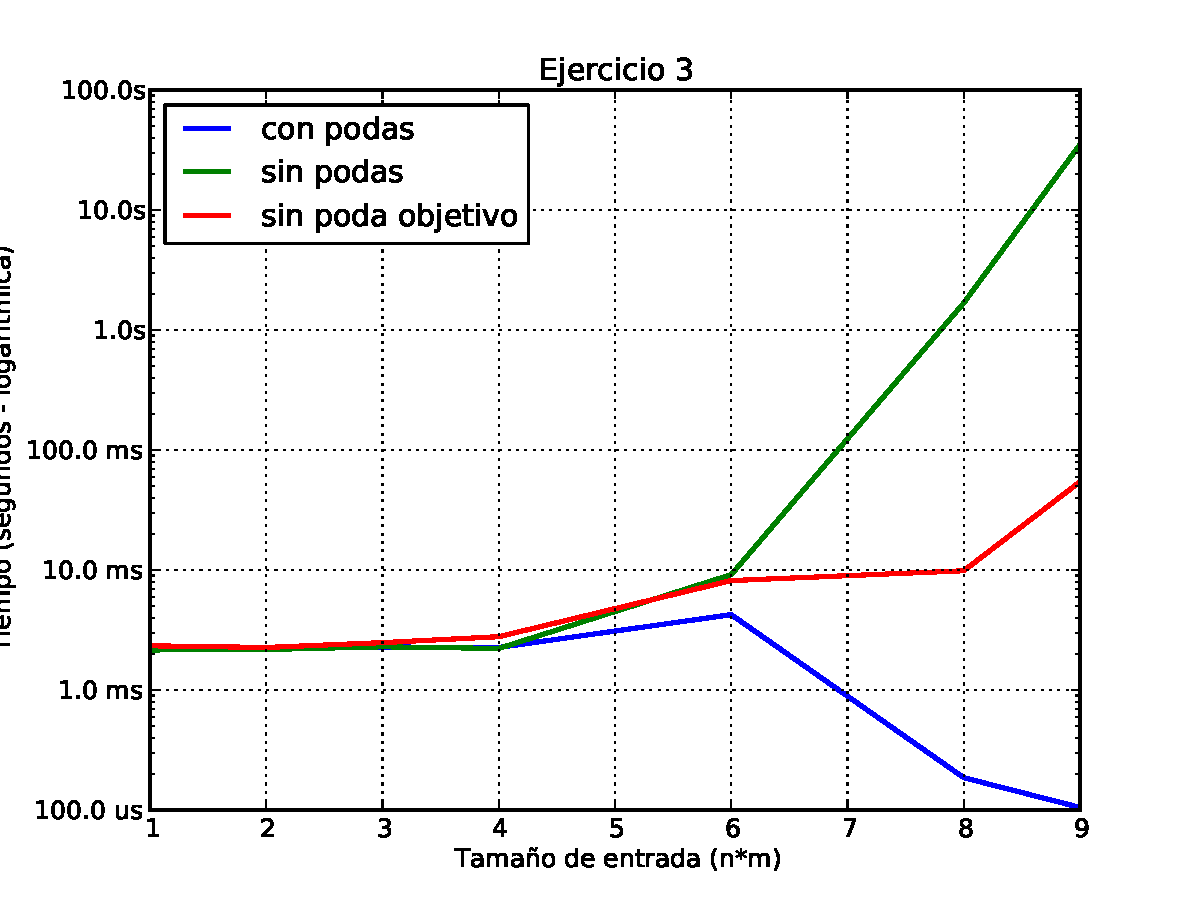
\includegraphics[width=1\textwidth,angle=0]{../ej3/graficos/test_sinPodas.pdf}
   \caption{Comparación de las podas}
   \label{fig:ej3-1}
   \end{center}
\end{figure}

Como se puede apreciar en el \textbf{\texttt{gráfico \ref{fig:ej3-1}}}, el cual
muestra el tamaño de entrada (n*m) en relación con el tiempo en segundos (en
escala logarítmica) el algoritmo presenta comportamientos parecidos ante
instancias de entrada pequeña, y las mismas se empiezan a diferenciar de forma
notoria a partir del tamaño de entrada 6. Todas las entradas utilizadas fueron
generadas de forma pseudoaleatoria. En el caso del caso ``sin podas'', se testeó
el Backtracking puro, es decir, sin ningún tipo de poda aplicada. Es notable ver
cómo ante un tamaño de entrada 9 (tablero de 3x3) el algoritmo sin podas tardó
aproximadamente un minuto. Se intentó testear para tamaños de entrada más
grandes, pero los tiempos de ejecución fueron muy grandes, por lo que no resultó
práctico realizar mediciones exploratorias para este tipo de tamaños. En el caso
de la medición ``sin poda objetivo'', se eliminó sólamente la poda sobre la
función de selección, la encargada de descartar las ramas que derivaran en
tableros imposibles. Así se puede apreciar una mejora notable en el rendimiento
del algoritmo frente a la versión sin podas. Tener en cuenta sobre todo la
escala logarítmica del \texttt{eje Y}, la cual implica que el algoritmo tardó
unas 1000 veces menos en relación al tiempo de ejecución sin podas\footnote{Dado
que el logaritmo es en base 10, una marca de línea punteada sobre el eje
representa un aumento de 10 veces sobre la marca anterior. Así, es fácil
calcular cuánto se diferencian los algoritmos}. En el caso del algoritmo ``con
podas'', se puede apreciar un descenso en el tiempo a partir del tamaño de
entrada 6. Esto podría parecer extraño, pero su explicación es que dada la forma
de la entrada, los tableros más pequeños resultaban imprácticos para la
aplicación de la poda, por lo cual el rendimiento del algoritmo era casi el
mismo con podas que sin podas. Luego, al crecer el tamaño del tablero, crece la
utilización de la poda, con lo cual parecería que el algoritmo tarda ``cada vez
menos''\footnote{Notar que su tope es en 100us, y no en 0.}. Si se pudiese
extender el análisis a tamaños mayores a 9, seguramente se podría ver cómo el
algoritmo crece luego de esa ``bajada''.



\begin{figure}[h]
   \begin{center}
   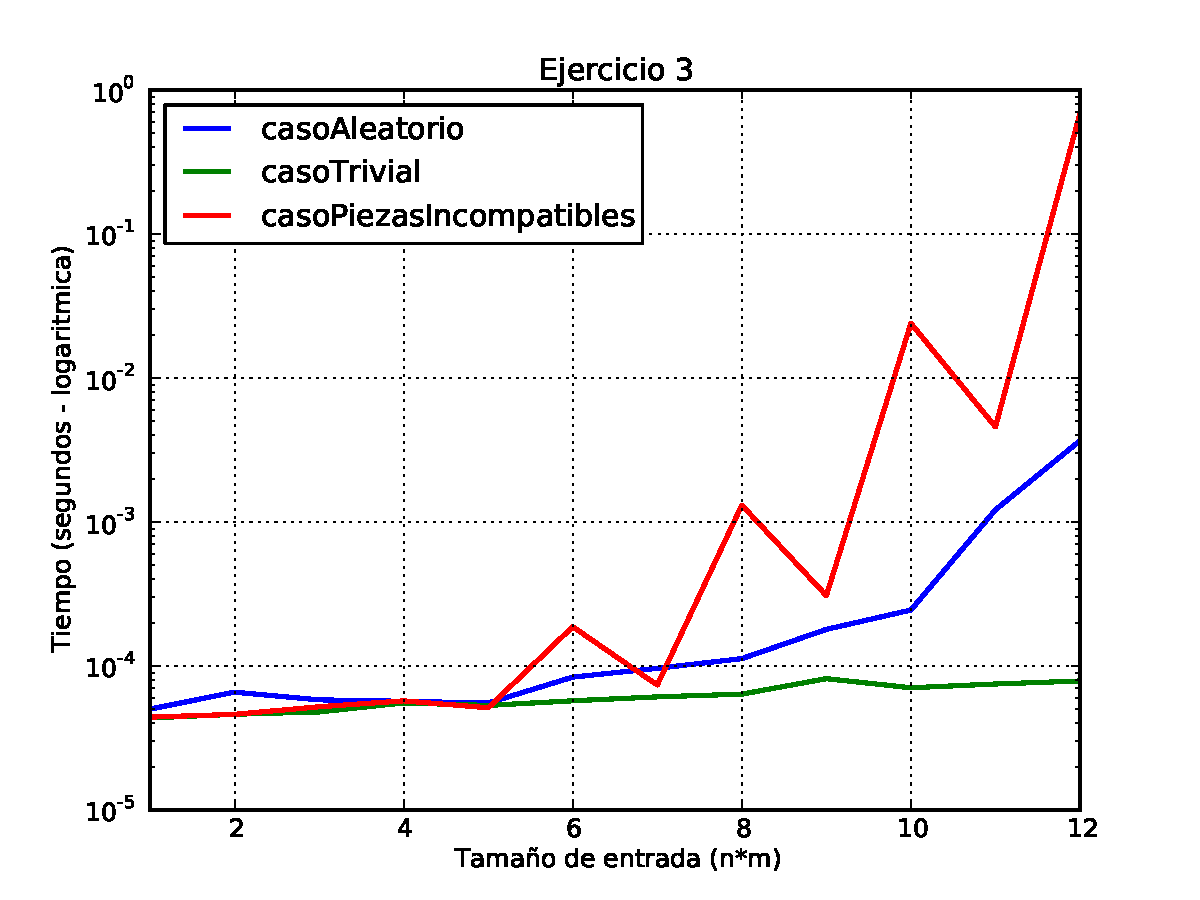
\includegraphics[width=1\textwidth,angle=0]{../ej3/graficos/test_exponencial.pdf}
   \caption{Comparación de la complejidad según el tipo de entrada}
   \label{fig:ej3-2}
   \end{center}
\end{figure}
\fixme{Explicar esto}

\begin{figure}[h]
   \begin{center}
   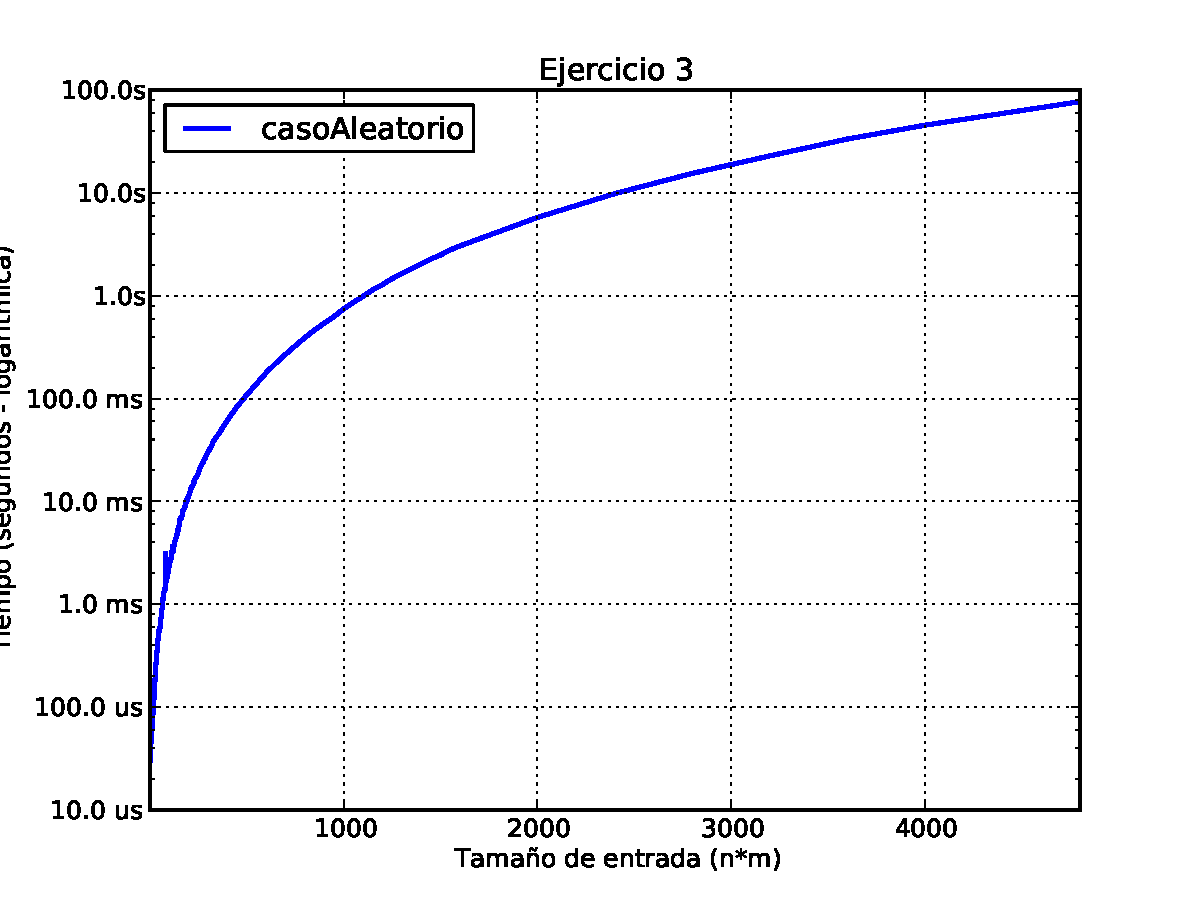
\includegraphics[width=1\textwidth,angle=0]{../ej3/graficos/test_con_podas.pdf}
   \caption{????????????????}
   \label{fig:ej3-3}
   \end{center}
\end{figure}
\fixme{Este test no iría por diferencias de criterio.}

\begin{figure}[h]
   \begin{center}
   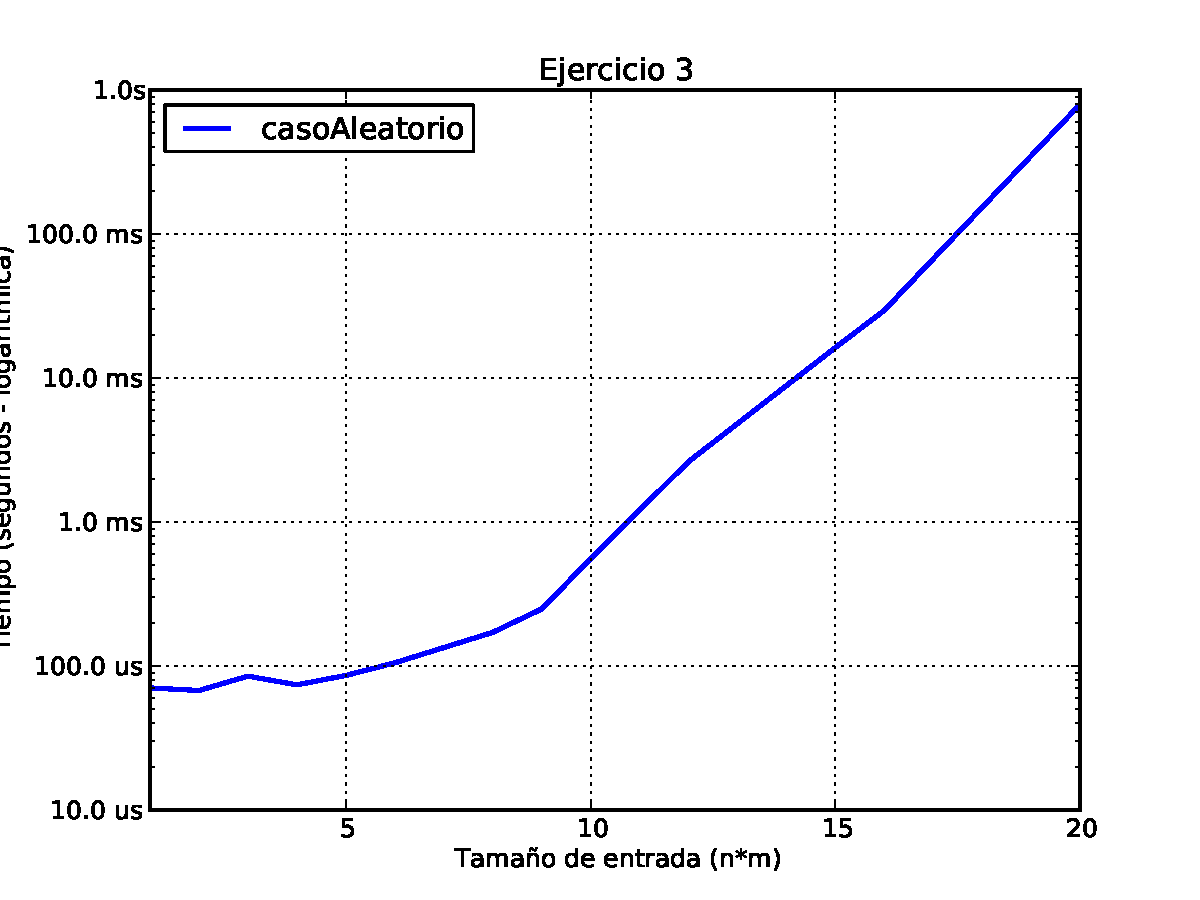
\includegraphics[width=1\textwidth,angle=0]{../ej3/graficos/test_normal.pdf}
   \caption{?????????????????}
   \label{fig:ej3-4}
   \end{center}
\end{figure}
\fixme{Explicar esto}

% -----------------------------------------------
\end{document}
